\documentclass[slovak,a4paper,11pt]{article}

\usepackage[utf8]{inputenc}
\usepackage{graphicx}
\usepackage{booktabs}
\usepackage{array}
\usepackage{paralist}
\usepackage{verbatim}
\usepackage{subfig}
\usepackage{amsmath}
\usepackage{index}
\usepackage{cite}
\usepackage[slovak]{babel}
\usepackage{fancyhdr}
\pagestyle{fancy}

\usepackage{sectsty}
\allsectionsfont{\sffamily\mdseries\upshape}

\usepackage[nottoc,notlof,notlot]{tocbibind}
\usepackage[titles,subfigure]{tocloft}
\renewcommand{\cftsecfont}{\rmfamily\mdseries\upshape}
\renewcommand{\cftsecpagefont}{\rmfamily\mdseries\upshape}

\title{Počítačové hry, ktoré učia programovať }
\author{Samuel Suja \\ ID: 111700}
%\date{}

\begin{document}
\maketitle
\tableofcontents

\begin{abstract}

Online vyučovanie sa v súčasnej situácií stalo nenahraditeľnou súčasťou študentského života. Niekedy však vedomosti zo školy nestačia na to, aby študenti vedeli všetko, čo potrebujú. V takom prípade je najlepšou možnosťou samoštúdium. Jednou z metód samoučenia je aj hranie počítačových hier. Napriek tomu že ich veľa ľudí berie ako stratu času, počítačové hry nás dokážu naučiť veci ako cudzie jazyky, logiku, históriu, a podobne. V tomto článku sa budeme venovať konkrétne takým počítačovým hrám, ktoré nás dokážu naučiť programovať, alebo nám aspoň vysvetliť základné princípy programovania. Zameriame sa na hry, ktoré sú založené na vykonávaní úloh pomocou písania alebo zoraďovania kódu, alebo ktoré obsahujú prvkypodobné samotnému programovaniu. Tými hrami budú ToonTalk, Human Resource Machine, Duskers, LightBot, ProBot, Scratch, Floorlab, Codingame, ktoré by mohli pomôcť začiatočníckym programátorom.

\end{abstract}

\section{Úvod}

More text.

\section{ToonTalk}
\subsection{Čo je ToonTalk?}
ToonTalk je programovací jazyk, ktorého kód môžeme vidieť v podobe interaktívneho animovaného sveta. K dispozícií máme prázdne pole a niekoľko objektov, ktoré je možné na toto pole umiestniť tak, aby sme z nich vytvorili funkčný program. Každý objekt má svoju vlastnú funkciu a zároveň dokáže komunikovať a spolupracovať s inými objektmi umiestnenými na poli. Animované nie sú len ikony týchto objektov, ale aj samotné činnosti ktoré vykonávajú a ich vzájomné vzťahy. V podstate celý proces fungovania programu je ukázaný na obrazovke a použivateľ môže v reálnom čase sledovať ako jeho program pracuje. \\
\begin{center}
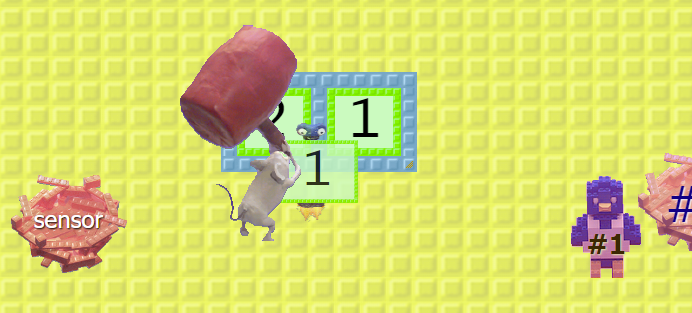
\includegraphics[scale=0.4]{toontalkmain}
\\ Obr. 1: ToonTalk v akcii: Myš zvyšuje číslo o 1
\end{center}
\subsection{Priebeh hry}
Základom ToonTalku sú samotné objekty, ktoré zastupujú príkazy a funkcie štandardných programovacích jazykov. Medzi ne patria:
\begin{itemize}
\item Čísla (Numbers) - slúžia ako vstupy do aritmetických operácií
\item Škatule (Boxes) - slúžia na ukladanie objektov
\item Vtáky a hniezda (Birds and nests) - vedia posielať správy
\item Váhy (Scales) - slúžia na porovnávanie objektov a hodnôt
\item Senzory (Sensors) - rozpoznávajú kliknutia alebo stlačenia kláves
\item Funkčné vtáky (Function birds) - vykonávajú funkcie so vstupnými škatuľami
\item Prehliadačové prvky (Browser elements) - umožňujú prácu s obrázkami a textom z iných webových stránok
\item Roboti (Robots) - vieme ich naučiť vykonávať prácu v našom programe
\end{itemize}
S týmito objektami vieme komunikovať a presúvať ich pomocou kurzoru, no máme k dispozícií dva ďalšie nástroje:
\begin{itemize}
\item Čarovná palička (A Magic Wand) - dokáže skopírovať objekty
\item Vysávač Dusty (Dusty the Vacuum) - slúži na odstraňovanie objektov z poľa
\end{itemize}
Cez hlavné menu ToonTalku sa dá dostať na webovú stránku, ktorá podrobne vysvetľuje ako všetky objekty fungujú, a zároveň poskytuje interaktívny návod na vyskúšanie funkčnosti všetkých objektov.
\subsection{Výhody a nevýhody}
Výhody:
\begin{enumerate}
\item ToonTalk umožňuje vidieť program v akcií: vidíme ako sa príkazy a funkcie vykonávajú v reálnom čase
\item Pre človeka, ktorý nikdy neprogramoval, je jednoduchšie vidieť ako jeho program funguje predtým ako to začne prepisovať do kódu
\item Objekty sa dajú rýchlo a jednoducho pridať, vymazať, alebo upraviť v pracovnom poli 
\item ToonTalk je zadarmo a dá sa spustiť cez skoro každý webový prehliadač bez potreby sťahovania
\item Správne naprogramovaný program môže slúžiť aj na naučenie iných vecí ako programovania
\end{enumerate}
Nevýhody:
\begin{enumerate}
\item Správne naprogramovať robotov je zložitejšie ako sa na prvý pohľad zdá. Pre ľudí, ktorí majú s programovaním skúsenosti, to môže byť zbytočne zdĺhavé
\item Zložitejšie programy je ťažké naprogramovať tak, aby všetko fungovalo bezchybne
\item Pri veľkom počte objektov je ťažké sa na poli zorientovať.
\item Poslednú aktualizáciu dostal ToonTalk na konci roku 2016, takže bugy, ktoré sa dodnes nachádzajú v aplikácií, nebudú už pravdepodobne nikdy odstránené
\end{enumerate}
\subsection{Zhodnotenie}
\section{LightBot}
\subsection{Čo je LightBot?}
LightBot nie je hra, ktorá dokáže hráčom priamo vysvetliť princípy programovania. Jadro tejto hry spočíva v skladaní príkazov do algoritmov s cieľom dostať sa do ďalšej úrovne. V hre ovláda hráč robota, ktorý sa vie pohybovať po políčkach a vykonávať rôzne úlohy. Aby hráč postúpil do ďalšej úrovne, musí pomôcť robotovi zapáliť svetlá na všetkých políčkach zafarbených modrou farbou. Toto hráč docieli poskladaním postupnosti príkazov do procedúry main, ktoré má robot vykonať aby úspešne dokončil úroveň. \\
\begin{center}
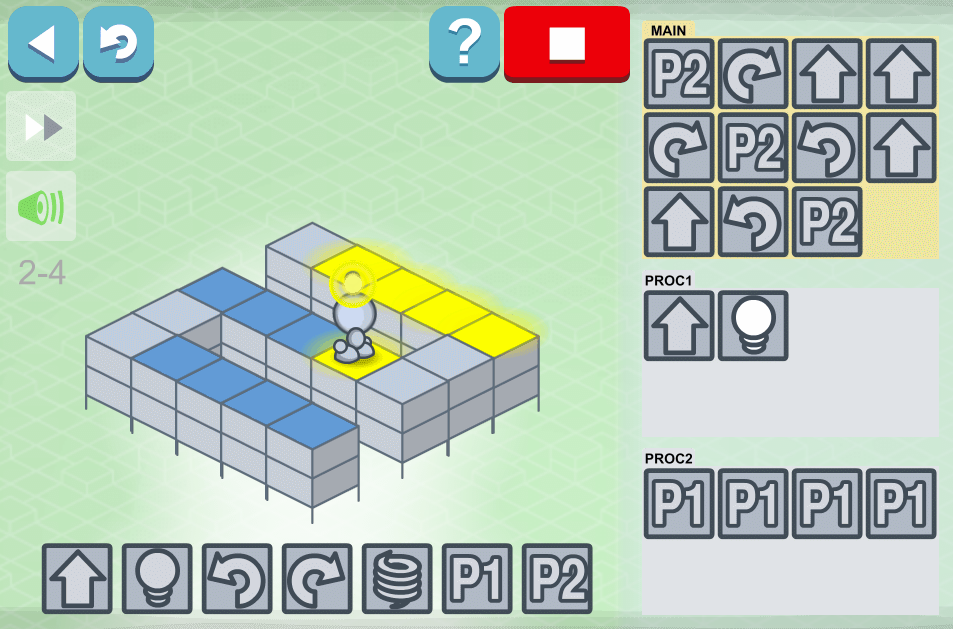
\includegraphics[scale=0.3]{lightbotmain}
\\ Obr. 2: Úspešné riešenie úrovne 2-4
\end{center}
\subsection{Priebeh hry}
Cieľom hráča je zapáliť všetky svetlá (políčka zafarbené modrou farbou) na hracom poli. Na pravej strane obrazovky sa nachádza procedúra main: po stlačení tlačidla na spustenie robota vykoná LightBot príkazy zadané v tejto funkcií. Main má však limit 12 príkazov, čo núti hráča v niektorých úrovniach nájsť to najefektívnejšie riešenie. V neskorších úrovniach pribudnú ďalšie procedúry, ktoré majú limit len 8 príkazov, ale môžeme ich vykonať cez procedúru main. To nám umožňuje vykonať niekoľkonásobne viac príkazov, ale zároveň robí riešenie úrovne zložitejším. \\
Na dolnej strane obrazovky sa nachádzaju samotné príkazy, ktoré môže robot vykonať. Medzi ne patrí:
\begin{itemize}
\item Pohyb dopredu
\item Zapálenie alebo zhasnutie svetla na políčku
\item Otočenie doľava
\item Otočenie doprava
\item Skok - špeciálny pohyb dopredu, ktorým sa dá pohybovať medzi políčkami rôznych výšok
\item Procedúra - vykoná všetky príkazy vo vybranej procedúre
\end{itemize}
\subsection{Výhody a nevýhody}
Výhody:
\begin{enumerate}
\item ToonTalk umožňuje vidieť program v akcií: vidíme ako sa príkazy a funkcie vykonávajú v reálnom čase
\item Pre človeka, ktorý nikdy neprogramoval, je jednoduchšie vidieť ako jeho program funguje predtým ako to začne prepisovať do kódu
\item Objekty sa dajú rýchlo a jednoducho pridať, vymazať, alebo upraviť v pracovnom poli 
\item ToonTalk je zadarmo a dá sa spustiť cez skoro každý webový prehliadač bez potreby sťahovania
\item Správne naprogramovaný program môže slúžiť aj na naučenie iných vecí ako programovania
\end{enumerate}
Nevýhody:
\begin{enumerate}
\item Správne naprogramovať robotov je zložitejšie ako sa na prvý pohľad zdá. Pre ľudí, ktorí majú s programovaním skúsenosti, to môže byť zbytočne zdĺhavé
\item Zložitejšie programy je ťažké naprogramovať tak, aby všetko fungovalo bezchybne
\item Pri veľkom počte objektov je ťažké sa na poli zorientovať.
\item Poslednú aktualizáciu dostal ToonTalk na konci roku 2016, takže bugy, ktoré sa dodnes nachádzajú v aplikácií, nebudú už pravdepodobne nikdy odstránené
\end{enumerate}
\subsection{Zhodnotenie}
\section{CodinGame}
\subsection{Čo je CodinGame?}
CodinGame
\subsection{Priebeh hry}
\subsection{Výhody a nevýhody}
\subsection{Zhodnotenie}
\section{CodeFights}
\subsection{Čo je CodeFights?}
\subsection{Priebeh hry}
\subsection{Výhody a nevýhody}
\subsection{Zhodnotenie}
\section{}

%\bibliography{referencie}
%\bibliographystyle{plain}

\end{document}
